\chapter{Politica de securitate}

Platforma \textit{MyBB} pune un accent foarte important pe securitate. Conform site-ului oficial, securitatea este cea mai mare proprietate. Cu toate acestea, dezvoltatorii sunt conștienți că orice e făcut de om este pasibil să conțină buguri / erori, de aceea au încercat să atragă utilizatorii să contribuie și ei la această latură. Au încercat să introducă un sistem de reward-uri, care la companiile mari se traduce în oferirea unei sume de bani în funcție de vulnerabilitatea submisă. Aici din păcate avem de-a face cu un proiect open source, un proiect în spate căruia nu există o companie, există doar ideea de voluntariat. Nu negăm că există o serie de oameni dispuși să doneze pentru o cauză, dar de multe ori aceste donații se reinvestesc în infrastructură în vederea menținerii proiectului online. Ca să nu o mai lungim foarte mult, cei care descoperă vulnerabilități și le raportează echipei MyBB vor fi trecuți pe o pagină onorifică a site-ului oficial - numită \textit{Security Hall of Fame}.

Este printre puținele platforme open source căreia i s-a făcut și un audit de securitate. Auditul a fost făcut în anul 2008, de către GulfTech. În urma acestui audit, s-a identificat câteva probleme și s-a putut trage concluzia că MyBB prezintă un low-risk record în ceea ce privește nivelul de securitate. Nici din punct de vedere istoric nu au fost găsite foarte multe high-risk vulnerabilități. De multe ori e important să înveți din greșeli, din problemele apărute de-a lungul timpului.

Tot de pe site-ul oficial - \textit{http://mybb.com}, se pot regăsi și câteva instrucțiuni pe care echipa MyBB le pune la dispoziție utilizatorilor. Până la urmă degeaba ai un sistem foarte sigur, dacă cei care îl administrează nu o fac corect. De aceea, trebuie cumva educați administratorii pentru a preîntâmpina diverse neplăceri mai târziu. Nu putem să le numim reguli. Ar fi doar niște recomandări. Le vom prezenta succint în paragrafele următoare.

\section{Actualizări periodice}

Utilizatorul trebuie să se asigure că are întotdeauna cea mai nouă versiune a platformei. Echipa MyBB este foarte proactivă și fixează o vulnerabilitate high-risk în cel mult 48 de ore. Numărul de actualizări pe an nu este foarte mare, o actualizare apare la un interval de 2-3 luni. Ce ar trebui să reținem aici? Faptul că actualizările sunt determinate în principiu de fixarea unei vulnerabilități importante sau introducea unui set major de feature-uri.

\section{Ascunderea versiunii platformei}

În ceea ce privește afișsarea versiunii curente a platformei, MyBB adoptă o politică diferită față de majoritatea competitorilor, în sensul în care în mod implicit versiunea platformei nu este afișată în subsol, alături de copyright. Cu cât cunoști mai puține lucruri despre un sistem, cu atât este mai greu să îl spargi. Asta nu înseamnă că administratorul nu are posibilitatea de a dezactiva acest comportament din panoul de administrare, dacă asta e ceea ce își dorește.

\section{Panoul de administrare}

Ca și majoritatea celorlalte platforme web, un forum oferă \textit{două interfețe}, o interfață de tip \textit{front-end} - forumul propriu-zis - unde predomină operațiunile de citire și un altă interfață de tipul \textit{back-end} - panoul de administrare - unde predomină operațiile de scriere. Din motive evidente, cea mai riscantă zonă din punct de vedere a securității o reprezintă cea de-a doua și anume panoul de administrare. O dată ce un utilizator a obținut acces la această zonă, el are control asupra întregului forum.

În acest sens, echipa MyBB ține să sublinieze faptul că panoul de administrare este doar pentru administratori. Celelalte grupuri de utilizatori nu au acces implicit la această zonă. Contează și numărul de administratori din sistem: \textbf{"More Admins = Less Security"}

Panoul de administrare trebuie ascuns, trebuie ținut la distanță de ceilalți utilizatori care nu au privilegii de administratori. De aceea ar fi bine să fie redenumit directorul în care se regăsesc sursele PHP pentru această zonă, din \textit{admin} în ceva mult mai bizar, folosind un string random. În acest caz, cel care pregătește un atac, sau are intenții mai puțin bune, trebuie să petreacă mai mult timp în descoperirea căii către panoul de administrare. Se poate merge și mai departe prin securizarea panoului de administrare folosind \textit{HTTP Basic Auth} cu o parolă adițională.

\subsection{Cod PIN}

\begin{wrapfigure}{r}{0.5\textwidth}
    \vspace{-60pt}
    \center{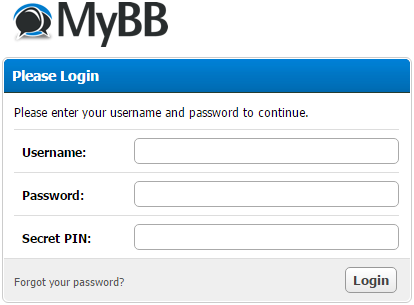
\includegraphics[width=0.5 \textwidth]{images/login.png}}
    \vspace{-20pt}
    \caption{\label{fig:Policy-AdminLogin} Autentificarea în AdminCP}
    \vspace{-10pt}
\end{wrapfigure}

Începând cu versiunea 1.8, în cadrul platformei s-a mai introdus un feature prin intermediul căruia se poate seta un cod PIN asupra panoului de administrare. Codul este format din 4 cifre și este static, putând fi modificat manual de administrator doar folosind accesul fizic la fișierele de configurare. Chiar dacă aduce un plus de securitate, prin cererea unor informații adiționale la autentificare, un dezavantaj ar fi faptul că acest cod nu se modifică automat după o perioadă de timp, modificările sale rămânând la latitudinea administratorului. În figura \ref{fig:Policy-AdminLogin} se poate observa existența acestui secret PIN.

\subsection{Backup-uri regulate}

Tot din panoul de administrare se poate configurare realizarea de backup-uri automate ale bazei de date la intervale periodice de timp. Procesul de backup este automatizat complet, arhiva rezultată putând fi păstrată pe server sau trimisă pe email, în cazul în care dimensiunea arhivei nu depășește 10 MB. Nu este necesar să facem un backup și la fișierele platformei pentru că acestea în mod normal ar trebui să fie recuperate ușor, fiind identice cu cele de pe site-ul oficial.

\section{Sistemul de modificări}

Platformei MyBB i se poate extinde funcționalitatea prin adăugarea unor modificări. Aceste modificări se numesc în termeni populari plugins. Sistemul de modificări funcționează prin intermediul interceptării unor evenimente ce au loc înainte sau după anumite acțiuni importante. Fiecare extensie, înregistrează la un dispatcher acțiunile pe care dorește să fie rulate atunci când un eveniment are loc. Așa după cum vă puteți da seama, fișierele de core nu sunt modificate sub nicio formă la instalarea unei noi modificări.

Comportamentul este puțin diferit față de ceea ce regăsim spre exemplu la platforma \textit{phpBB}, în care instalarea unei modificări presupune modificare unui sau mai multor fișiere din core. În cazul nostru, avantajul este reprezentat de faptul că fișierele de core rămân intacte, dezavantajul fiind introducerea unui overhead prin faptul că există un număr mai mare de apeluri de funcții. Se poate spune că securitatea este sporită în detrimentul performanței!

\newboxedtheorem[boxcolor=none, background=blue!5, titlebackground=blue!20, titleboxcolor = none]{theo}{Studiu de caz}{anything}
\begin{theo}[Număr de modificări utilizate]
Cu cât numărul de modificări instalate pe o platformă MyBB este mai mic cu atât riscurile în apariția unor vulnerabilități este mai mic. Momentan nu există o metodă prin care modificările realizate de către alți developeri să fie testate riguros, motiv pentru care acestea pot mai avea scăpări, introducând diverse probleme de securitate.\\
\textbf{Concluzie:} La ora actuală cele mai mari probleme de securitate au fost cauzate de tot felul de modificări.
\end{theo}

O să vedem un pic mai târziu ce face comunitatea oficială pentru a reduce numărul de modificări cu probleme de securitate.

\section{Controlul accesului în sistem}

TODO - Aici trebuie să vorbim despre grupurile de utilizatori.

\section{Filtrarea informației}

TODO - Aici trebuie să vorbim despre cum este tratată informația din mediul extern. ce se face pentru a evita injectarea de cod?

\section{Sesiuni și parole}

TODO

\section{Interacțiunea cu comunitatea oficială - \textit{MyBB.com}}

TODO